\chapter{\acrlong{rc}}
\label{rc}

\section{Introduction}


% What is a rc
\gls{rc} is a bio-inspired artificial \gls{rnn} which is based on the \gls{esn} introduced by Herbert Jaeger in \cite{Jaeger2004}. This computation scheme is well suited for real-time data processing and for chaotic time series prediction\cite{Jaeger2004, JaegerH.2001Tesa, Lukoeviius2012}, and achieves state of the art performances in those domains, as well as in speech recognition\cite{Verstraeten2006, NIPS2010_4056, Jaeger2007}, nonlinear channel equalisation\cite{Jaeger2004} and financial forecasting \cite{financialTimeSeries}.\\

% nn
A \gls{rcer} is specific kind of \gls{nn}, which is a computation paradigm mimicking the behaviour of a biological brain. As can be seen on Figure \ref{nn}, the artificial neurons are merely interconnected entities carrying an activation level. As shown on Figure \ref{nn-update}, the activation level of a neuron is updated according to the connection weights of the network, also known as the synaptic matrix, and with a nonlinear function, called the \textit{activation function}, which allows \gls{nn} to perform classification tasks \cite[p.225]{bishop2006pattern}\cite[p.727]{russell2010artificial}.\\

\begin{figure}[h]
	\centering
	\begin{subfigure}{.5\textwidth}
		\centering
		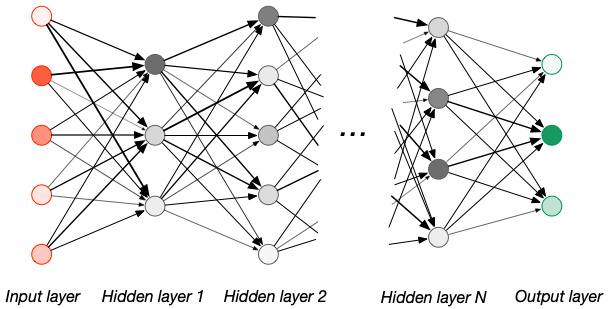
\includegraphics[height=3.5cm]{nn.png}
		\caption{High-level overview a feedforward \gls{nn}. Input data is fed into input neurons, and the result of the computation is read on the activation level of output neurons. \\ \cite[p.228]{bishop2006pattern}}
		\label{nn}
	\end{subfigure}%
	\begin{subfigure}{.5\textwidth}
		\centering
		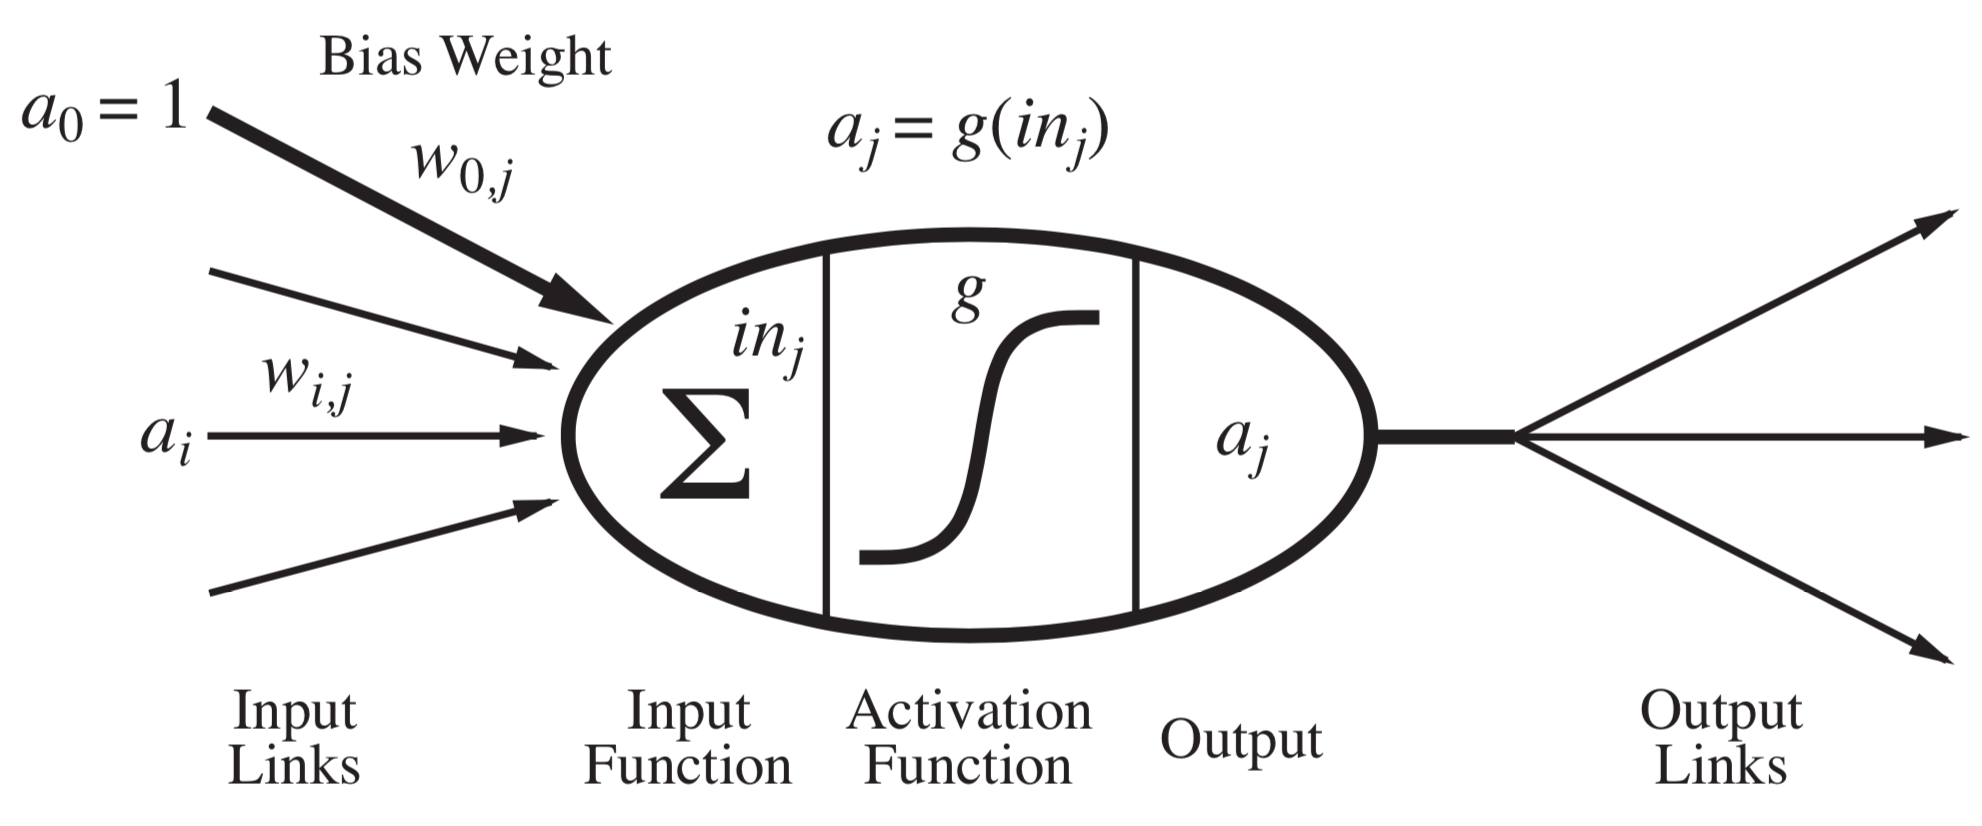
\includegraphics[height=3.5cm]{nn-update.png}
		\caption{Update of the activation level of a neuron. The activation level of the neurons from the previous layer are linearly combined through the input links, and a nonlinear function is applied to the result of the sum.\\ \cite[p.728]{russell2010artificial}}
		\label{nn-update}
	\end{subfigure}
	\caption{\acrlong{nn} seen from different points of view}
\end{figure}

% Principle of rc
The activation level of the neurons making up the reservoir characterise its state, which is a time-dependent object. The neurons are interconnected in such a way that they influence the dynamic of each other, leading to a complicated evolution of the state of the reservoir. What a first glance may seem to be a mathematical nightmare turns out to be the main advantage of \gls{rc}. Indeed, when the reservoir is properly set up, the activation level of each of the neurons becomes a systematic transformed version of the input signal \cite{Jaeger2004}. This is called the echo state and this is the regime where \gls{rcer} reach their best performance. This is due to the fact that this is an operating point where the transients caused by the inputs are neither amplified nor damped, somehow providing a memory to the reservoir \cite{Goudarzi2014ACS, JaegerH.2001Tesa}. The output of a \gls{rcer} is obtained by adequately combining the activation state of each neurons. The ideas developed in this paragraph are illustrated on Figure \ref{rc_principle}.\\

\begin{figure}[h]
	\centering
	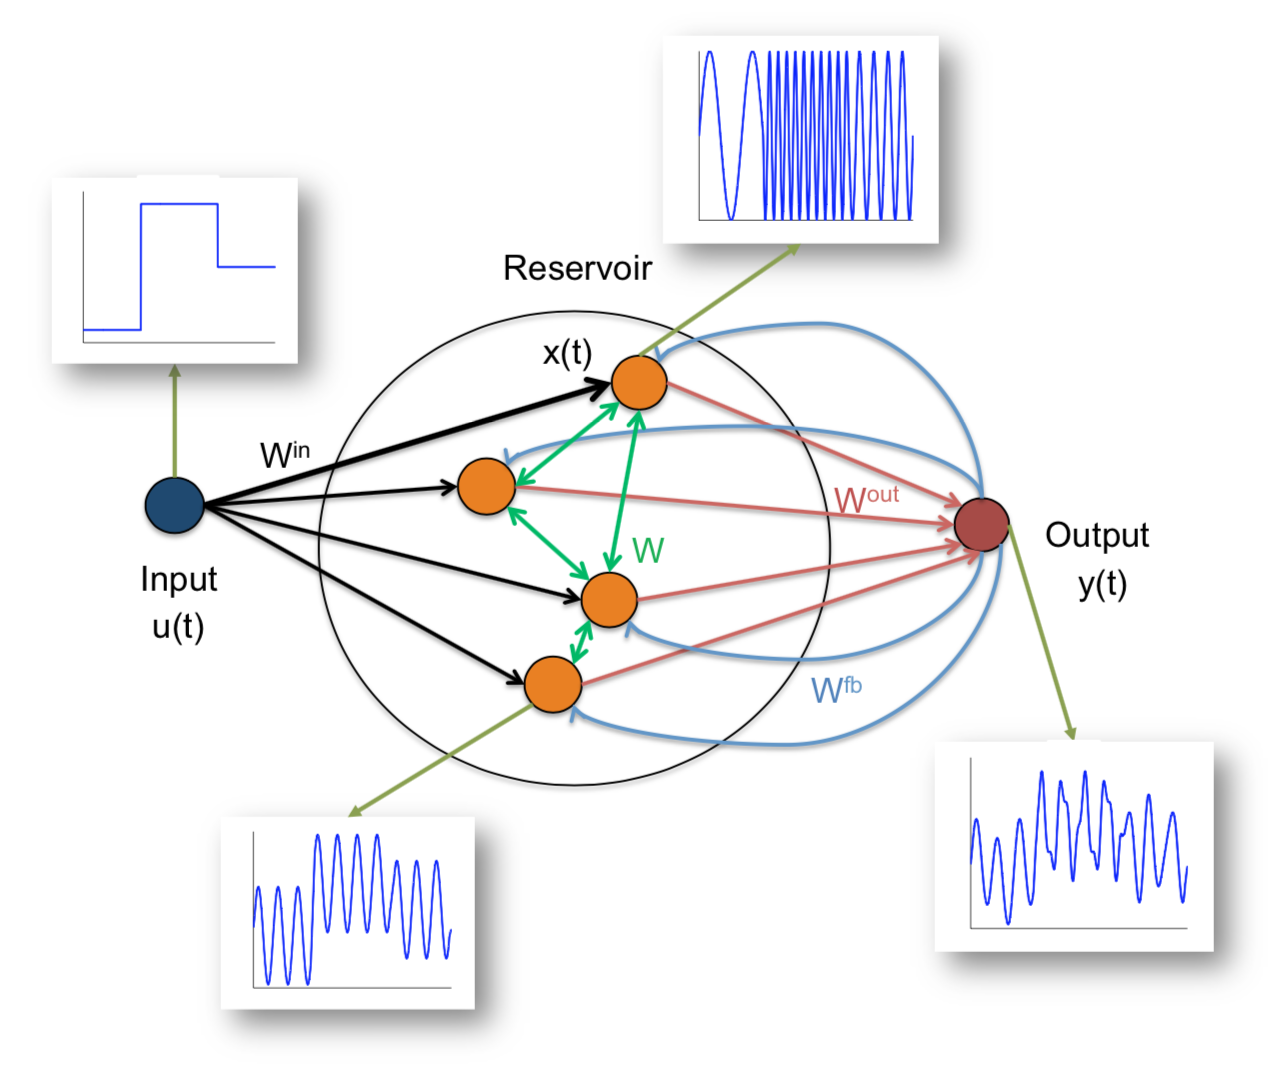
\includegraphics[width=.6\textwidth]{rc_principle.png}
	\caption{Principle scheme of a \acrlong{rcer} \cite{financialTimeSeries}}
	\label{rc_principle}
\end{figure}

% ML - sources
Regardless of the learning scheme used to train a \gls{nn}, the basic idea is always to minimise the difference between the desired and the actual outputs. In practice, this is achieved by updating the coefficients in the synaptic matrix of the \gls{nn} \cite[p.233]{bishop2006pattern}\cite[p.733]{russell2010artificial}. On Figure \ref{nn-ml}, the learning procedure for a small portion of a feed-forward \gls{nn}, for instance the one from Figure \ref{nn}, is shown. The \gls{nn} is fed with data from the left, as can be seen with the blue arrows. The red arrows represent the error on the output being \emph{backpropagated}, which means that the learning algorithm evaluates how each connection weight of the synaptic matrix should be updated in order to decrease the output error \cite[p.241]{bishop2006pattern}. This procedure often turns out to be a really complicated task, which explains why the development of efficient \gls{ml} algorithms is such a hot topic nowadays. On the other hand, as can be seen on Figure \ref{rc-ml}, \gls{rcer} only need their output weights to be adjusted when being trained, which makes them computationally lighter\cite{Jaeger2004}. This is due to the fact the connections of the reservoir should not contain any information about the task, but should only be used to reach the \gls{esn} regime, as previously mentioned. There are two main families of training methods for \gls{rcer} \cite{Jaeger2002}. On the one hand, there is the \textit{batch learning}, which comprises the methods requiring to first store a bunch of data regarding the task being taught before being able to actually compute the output weights. Once enough data is gathered, this kind of algorithms returns the optimal weights all at once. They present the advantage of involving only one training phase, after which the \gls{rcer} are ready to perform. However, the need for vast amount of data and the inability for the \gls{rcer} to adapt to an input evolving out of the range for which it has been trained are two drawbacks. On the other hand, \textit{online learning} methods allow to iteratively improve the output weights. Therefore, starting from a first guess, these algorithms will converge to workable output weights. They are much more adaptable than the batch learning ones, however, their convergence is not guaranteed and can be slow \cite{JaegerTraining, schrauwen}.

\begin{figure}[h]
	\centering
	\begin{subfigure}{.5\textwidth}
		\centering
		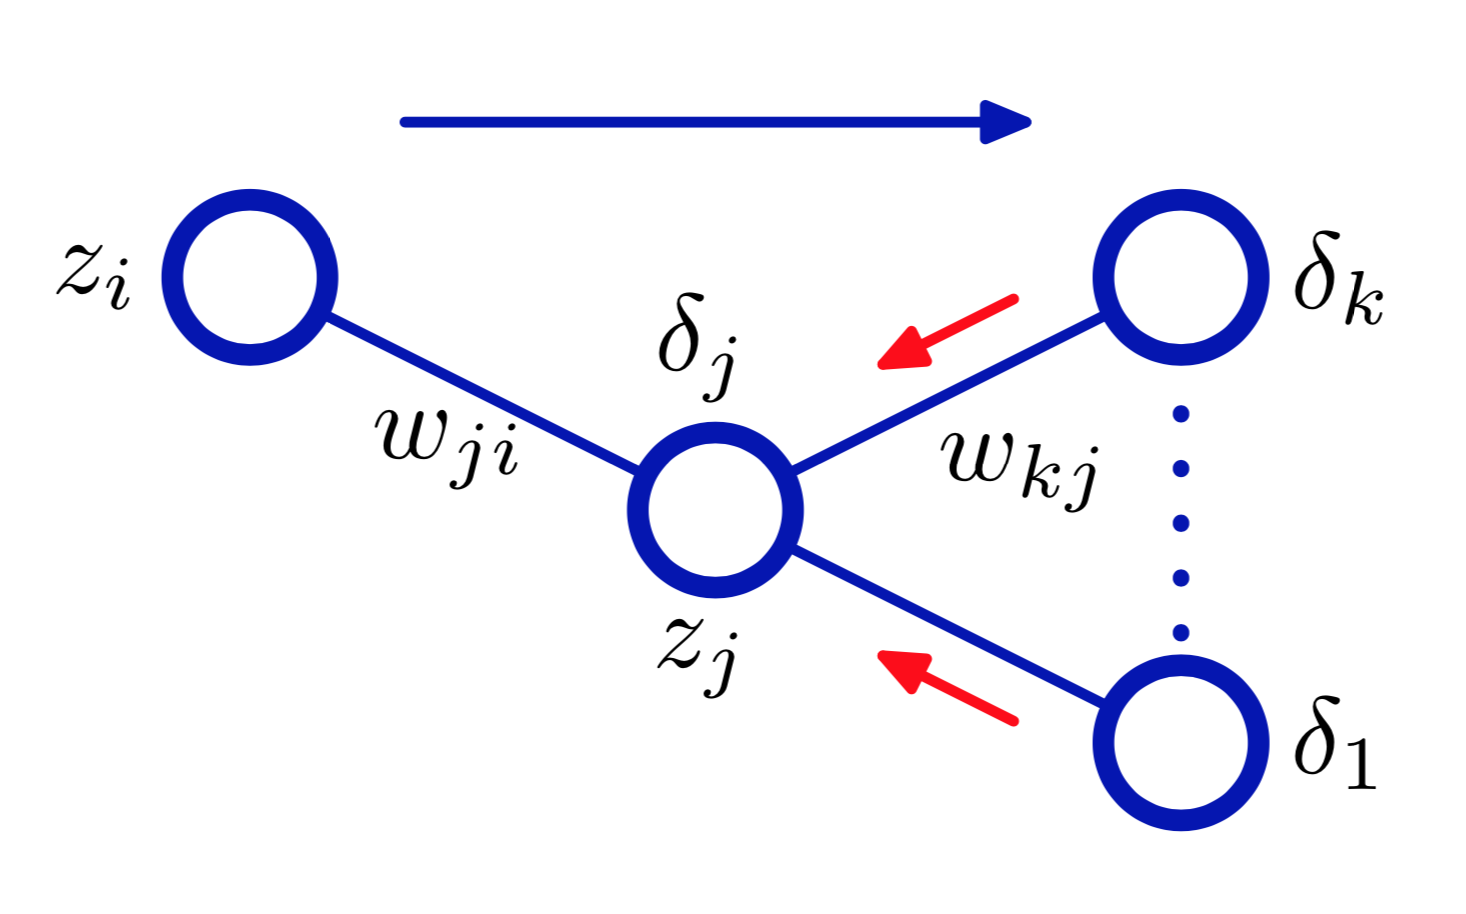
\includegraphics[height=3.5cm]{nn-ml.png}
		\caption{\acrlong{nn} \cite[p.244]{bishop2006pattern}}
		\label{nn-ml}
	\end{subfigure}%
	\begin{subfigure}{.5\textwidth}
		\centering
		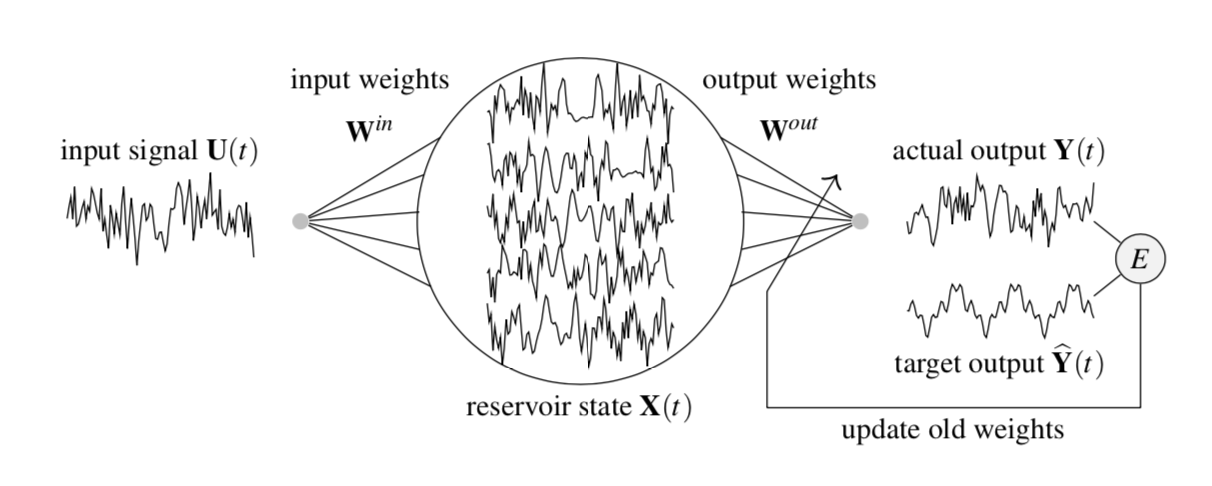
\includegraphics[height=3.5cm]{rc-ml.png}
		\caption{\acrlong{rcer} \cite{Goudarzi2014ACS}}
		\label{rc-ml}
	\end{subfigure}
	\caption{\acrlong{ml} for different kinds of \acrlongpl{nn}}
\end{figure}

In order to reach the echo state regime, the constraints on the coupling between the neurons of the reservoir are actually quite loose. What is required is to introduce randomness and to break symmetries in the synaptic matrix. Once this condition is verified, the performance of the reservoir can be modified by tweaking only a small set of variables applying to the whole \gls{rcer}. In other words, as soon as the basic structure of the reservoir is set, there is no need to individually change the value of each connection to improve it, only modifying globally the reservoir is enough, for example by multiplying all the connection weights by the same constant. This property is a key element of the \gls{rcer} paradigm that allows it to be implemented in physical systems other than classical, silica-based computers. This has already been done several times in photonic experiments, leading to the novel concept of \gls{prc}. Different implementations have been proposed: fully integrated photonic chips \cite{Vandoorne2014}, fibre-based systems with time-multiplexed neurons coupled through a delay line with nonlinearities introduced by a Mach-Zehnder intensity modulator \cite{Paquot2012, Antonik2017, Duport2016}, by saturation of absorption \cite{Dejonckheere2014, Vandoorne2008} and by the readout photodiodes \cite{Vinckier2015}. This latter configuration even reached state of the art performances in different benchmark tasks, such as Memory Capacity Evaluation, \acrshort{narma}10 (\acrlong{narma} of order 10), nonlinear channel equalisation, and isolated spoken digit recognition. In \cite{Fernando2003}, the researchers even manage to perform speech recognition and the XOR task\footnote{The XOR task consists in reproducing the behaviour of a logical XOR gate, which is a task of historical importance for \gls{nn} \cite{minsky1969perceptrons}.} in a bucket of water. 

\section{Mathematical Model}

In this section, an overview of the mathematical framework linked to \gls{rc} is given. First, let us define the \textit{state} of the reservoir. As said previously, the \gls{rc} can be fully described by the activation level of each of its neurons. The state is therefore defined as a vector whose components are the activation levels of the neurons. If the number of neurons making up the reservoir is $N$, and if $x_i$ is the activation level of the $i^{\text{th}}$ neuron, the the state vector reads as follows:

\begin{equation}
	\mathbf{x} = \begin{bmatrix}
		x_1\\
		\vdots \\
		x_i \\
		\vdots \\
		x_N
	\end{bmatrix}
\end{equation}

\newpage

The dynamics governing the state vector and the output of the reservoir proposed in \cite{JaegerH.2001Tesa} are presented below. In practice, it is too general for the implementations studied in this work. However, the equations are introduced without loss of generality, and simplifying assumptions will be specified later.

\begin{align}
	\mathbf{x}(n+1) &= \mathbf{f} \left( \mathbf{W}^{\text{in}} \mathbf{u}(n+1) + \mathbf{W} \mathbf{x}(n) + \mathbf{W}^{\text{fb}} \mathbf{y}(n) \right) \label{rc_dynamics}\\
	\mathbf{y}(n+1) &= \mathbf{f}^{\text{out}} \left( \mathbf{W}^{\text{out}} \left(\mathbf{x}(n+1), \mathbf{u}(n+1), \mathbf{y}(n)\right) \right) \label{rc_output}
\end{align}

Different elements need to be defined: 

\begin{itemize}
	\item $n \in \{1, \dots, T\}$ is the discrete time variable
	\item $\mathbf{u} \in \mathbb{C}^k$ is the input vector which enters the reservoir through the input neurons
	\item $\mathbf{W}^{\text{in}} \in \mathbb{C}^{N \times k}$ is the input matrix. It indicates how the $k$ input neurons are connected to the neurons of the reservoir
	\item $\mathbf{x} \in \mathcal{S} \subseteq \mathbb{C}^{N}$ is the state vector, as said previously
	\item $\mathbf{W} \in \mathbb{C}^{N \times N}$ is the synaptic matrix, or the connection matrix which has already been introduced
	\item $\mathbf{y} \in \mathbb{C}^{m}$ is the output vector of the reservoir whose value can be read out on the output neurons
	\item $\mathbf{W}^{\text{fb}} \in \mathbb{C}^{N \times m}$ is the feedback matrix. It couples the output back into the reservoir
	\item $\mathbf{f}: \mathbb{C}^N \mapsto \mathcal{S}$ is the nonlinear function mapping the linear combination it receives as argument to a valid state vector
	\item $\left(\mathbf{x}(n+1), \mathbf{u}(n+1), \mathbf{y}(n)\right)$ is the concatenation those three vectors
	\item $\mathbf{W}^{\text{out}} \in \mathbb{C}^{m \times (N+k+m)}$ is the output matrix of the reservoir. It is optimised through \gls{ml}
	\item $\mathbf{f}^{\text{out}} : \mathbb{C}^{m} \mapsto \mathbb{C}^{m}$ is the output function of the reservoir
\end{itemize}

\subsection{Simplifying assumptions for Optical \acrshort{rcer}}

In what follows, the input and the output of the reservoir are just scalar values, which simplifies the previous equations. Thus, $\win$ becomes a simple real vector of length $N$ which is called the \textit{input mask} $\mathbf{m}$ in the literature. The input mask can be chosen in different ways: in \cite{Duport2016}, they use a sinusoidal input mask whereas in \cite{Antonik2017, Vinckier2015, Paquot2012} the input masks are randomly chosen. Once this vector is fixed, it should be multiplied by a constant to optimise the performance of the \gls{rcer}. Very few constraints apply to the creation of the connection matrix $\w$. It can be randomly generated and sparse. However, to make the occurence of the echo state more likely to happen, one wants to work with a spectral radius $\rho \left( \w \right)<1$. If this condition is not verified, as well as degrading the performance of the reservoir, this can also lead to instabilities \cite{Lukoeviius2009}. Therefore, once again, once the matrix $\w$ is fixed, one can multiply it by another constant for the same reason mentioned before. Thus, by defining $\alpha$ and $\beta$,  the feedback\footnote{This may seem like a misnomer at this point since it has nothing to do with $\wfb$, but this name is used because $\alpha$ acts as a gain for the activation level of the neurons being fed back into the reservoir.} and input gains, respectively:

\begin{equation}
	\w \longrightarrow \alpha \mathbf{A}, \quad \win \longrightarrow \beta \mathbf{m}
\end{equation}

This is an example of what was introduced in the previous section. Indeed, the difficulty of tweaking each and every coefficients in order to improve the reservoir is transferred to just a few global variables. This is of great practical importance for physical implementations of \gls{rcer}. Indeed, the experimentalist can alter the behaviour of its \gls{rcer} by only modifying a few global experimental variables.\\

In practice, the feedback of the reservoir output is neglected, especially for physical implementations, so $\wfb$ should be null. Also, the concatenation is not observed. Indeed, in general, when computing the output, only state vectors are considered. Speaking of them, they belong to $\mathcal{S}$ because the fact that the functions $\mathbf{f}$ used in practice are bounded, so the vectors $\mathbf{x}$ span a space \textit{smaller} than $\mathbb{C}^N$. The simplified version of the previous equations reads:

\begin{align}
	\mathbf{x}(n+1) &= \mathbf{f} \left( \alpha \mathbf{A} \mathbf{x}(n) + \beta \mathbf{m} u(n+1) \right)\\
	y(n+1) &= f^{\text{out}} \left( \mathbf{W}^{\text{out}} \mathbf{x}(n+1) \right)
\end{align}

As far as \gls{prc} are concerned, two approaches to determine the functions $\mathbf{f}$ and $f^{\text{out}}$ are followed in the literature. The first kind of \gls{prc} are those using optical components exhibiting nonlinear behaviour, such as Mach-Zehnder intensity modulators \cite{Duport2016, Paquot2012, Antonik2017}, semiconductor optical amplifiers \cite{Vandoorne2008} or semiconductor saturable absorber mirror \cite{Dejonckheere2014} to couple the neurons. In an actual optical experiment, the measurements have to be done with photodiodes. These devices can only inform about the intensity of the light, which is the squared modulus of the phaser representation of the electric field, and not about the actual electric field. However, in the scheme presented above, the input and the activation level of the neurons are real objects appropriately encoded in the intensity of the light, and can therefore be directly read out by a photodiode, hence this simple expression for the output of the reservoir:

\begin{equation}
	y(n+1) = \sum_{i=1}^{N} W^{\text{out}}_i x_i (n+1)
	\label{lin_output_rc}
\end{equation}

On the other hand, in \cite{Vinckier2015}, the neurons are encoded in the complex phaser representation of the electric field and are linearly coupled using a delay line. This scheme is a linear reservoir:

\begin{equation}
	\mathbf{x}(n+1) = \alpha \mathbf{A} \mathbf{x}(n) + \beta \mathbf{m} u(n+1)
	\label{rc_lin_dynamics}
\end{equation}

Therefore, it appears more clearly why the condition mentioned previously regarding $\rho \left( \alpha \mathbf{A} \right)$ is relevant. Indeed, if $\mathbf{x}_j$ is an eigenvector of $\alpha \mathbf{A}$ with eigenvalue $\lambda_j>1$, the above equation will lead to an exponential divergence $\mathbf{x}_j(n) \sim \lambda_j^n \mathbf{x}_j(0)$. On the other hand, if $\lambda_j$ is too small, the state $\mathbf{x}_j$ will be damped too quickly, deteriorating the memory capabilities of the reservoir and preventing it from reaching the echo state. In the linear reservoir, since the neurons and the input are inscribed in the complex electric field, the nonlinearity is introduced by the read out photodiodes. The output is therefore given by:

\begin{equation}
	y(n+1) = \sum_{i=1}^{N} W^{\text{out}}_i |x_i (n+1)|^2
	\label{quad_output_rc}
\end{equation}

The latter scheme is of particular interest for the remaining of this work, because the novel proposed implementation relies on the sme principle. It is also interesting to notice that is quite similar to the first \gls{nn} paradigm, the \emph{perceptron}, introduced by F. Rosenblatt in 1958 \cite{Rosenblatt58theperceptron}. Equations \eqref{lin_output_rc} and \eqref{quad_output_rc} give an interesting intuition on the meaning of the \gls{esn}. Indeed, as said previously, when a \rc reaches the echo state, each of the neurons tends to systematically reproduce a modified version of the input, the actual modification being an individual characteristic of each neuron \cite{Jaeger2004}. One can see this feature in the perspective of linear algebra. When the \rcer is fed with an input, it creates a set of time varying functions that can intuitively be seen as a basis in which one can try to express the output of the reservoir, which is nothing but a vector in the vectorial space of functions. This is why it is often said in the literature that a \rcer maps an input to a higher dimensional space. Therefore, one can in theory approach any target function with an arbitrary precision, depending on the number of neurons in the reservoir \cite{Jaeger2004}. The higher the number of neurons, the closer to a genuine series development one gets. Still in the same perspective, the $W^{\text{out}}_i$ can be seen as the Fourier coefficients of the output function.\\

To determine the output matrix $\mathbf{W}^{\text{out}}$, as said in the previous section, there exists several techniques, but the underlying intuitive idea is always the same. One wants to minimise the deviation between the actual output and the target. Different metrics can be used to encapsulate the distance between those values. In the literature, one of the most frequent is the NMSE, for Normalised Mean Square Error:

\begin{equation}
	\text{NMSE} = \frac{\langle \| \hat{\mathbf{y}}(n) - \mathbf{y}(n)\|^2 \rangle _n}{\langle \| \hat{\mathbf{y}}(n) - \langle \hat{\mathbf{y}}(n) \rangle _n \|^2 \rangle _n}
\end{equation}

With $\hat{\mathbf{y}}(n)$ the target vector, $\langle \dots \rangle _n$ the average with respect to $n$, and $\| \dots \|$ the euclidean norm \cite{Duport2016}. Different optimisation algorithms can be used for the optimisation in practice, but their description is out of the scope of this work, see \cite{Lukoeviius2009} for more details.

\section{Simulations}

In this section, two different benchmark tasks on which \rcer are evaluated are briefly introduced, and then the results obtained in numerical simulations are shown. Both of them are implementations of the discrete model described in \cite{Vinckier2015}, which is the linear reservoir with the quadratic output for which an overview was given in the previous section:

\begin{equation}
	x_i(n+1) = 
	\begin{cases}
		\alpha e^{j\phi} x_{i-k}(n)+\beta \left(m_i u(n) +A_0 \right) & \text{if } k \leq i \leq N\\
		\alpha e^{j\phi} x_{N+i-k}(n-1)+\beta \left(m_i u(n) +A_0 \right) & \text{if } 0 \leq i \leq k			
	\end{cases}
\end{equation}

Here, the $\text{i}^{th}$ neuron is sent to another one at each update of the state vector, with $k$ being the detuning parameter determining to which one it is mapped. $e^{j\phi}$ is the phase acquired by the complex electric field when it propagates in the delay line. $A_0$ is the input bias.

\subsection{\gls{narma}10}

\acrlong{narma} of order 10 is a model often used because it exhibits a similar behaviour to that of a time series \cite{Paquot2012}. If $u(n)$ is a random variable uniformly distributed along the interval $[-0.5, 0.5]$, the recurrent equation for \gls{narma}10 reads:

\begin{equation}
	\hat{y}(n+1) = 0.3\hat{y}(n)+0.05y(n)\left(\sum_{i=0}^9 y(n-i) \right)+1.5u(n-9)u(n)+0.1
\end{equation}

\begin{figure}[h]
	\centering
	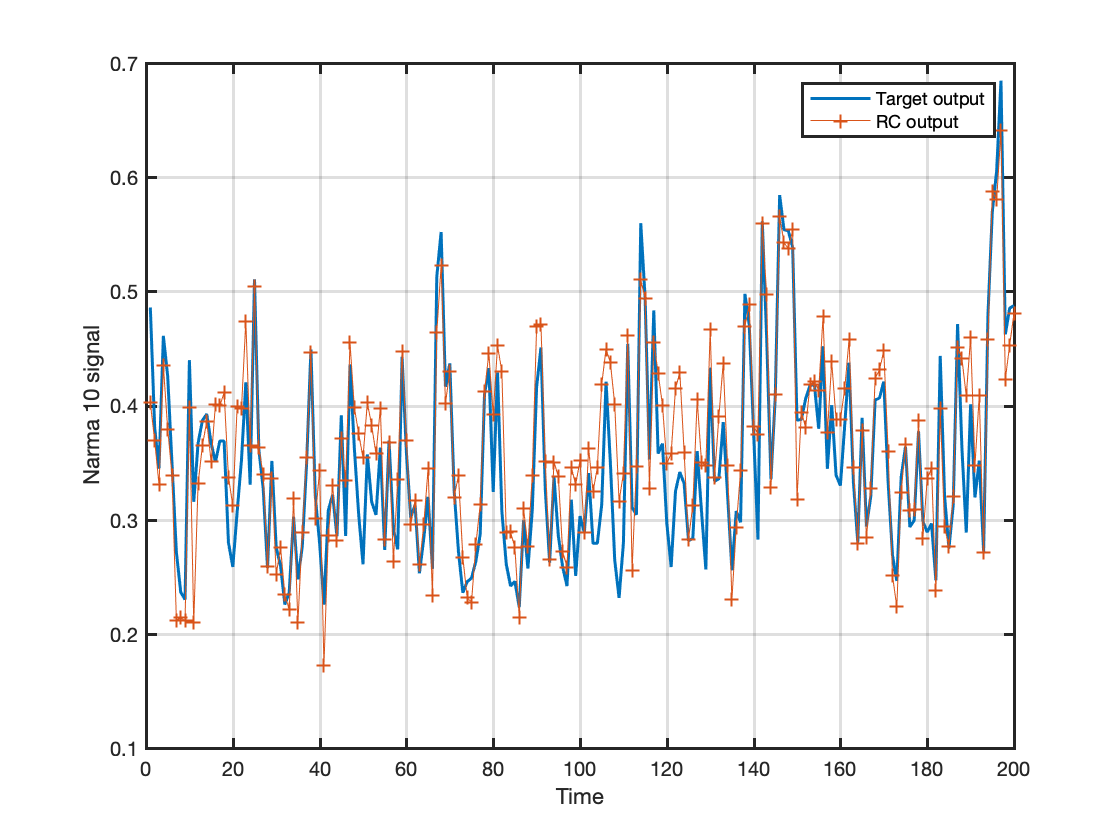
\includegraphics[width=\textwidth]{narma10.png}
	\caption{\gls{narma}10 task with NMSE equal to 0.1541. This reservoir is made of 50 neurons. $\alpha=0.5$, $k=7$, $\phi=0$ rad, $\beta=1$, $A_0=1$, $\mathbf{m}$ is a random vector distributed between 0 and 1. The first 300 time steps were discarded in order to let enough time to the reservoir to enter the echo state (washout). Then the reservoir was trained for 3000 time steps and tested over 6000 time steps. This reservoir is particularly well suited for  \gls{narma}10 since the nonlinearities in the signal are mostly quadratic \cite{Vinckier2015}.}
	\label{narma10}
\end{figure}

\subsection{Nonlinear channel equalisation}

This task consists in the reconstruction of a signal after it has travelled through a nonlinear channel. The emitted signal $\hat{y}$ is randomly drawn from the symbol set $\{-3,-1,1,3\}$. It is first superposed with following and preceding symbols as can be seen in \eqref{signal_mixing}. After that, a nonlinear transformation is applied to the mixed signals, and a Gaussian noise, whose intensity can be set in order to adjust the signal to noise ratio, is added in \eqref{nonlinear_ch}. 

\begin{align}
	q(n) &= 0.08\hat{y}(n+2)-0.12\hat{y}(n+1)+\hat{y}(n)+0.18\hat{y}(n-1) \nonumber\\
	&-0.1\hat{y}(n-2)+0.091\hat{y}(n-3)-0.05\hat{y}(n-4) \nonumber\\
	&+0.04\hat{y}(n-5)+0.03\hat{y}(n-6)+0.01\hat{y}(n-7) \label{signal_mixing}
\end{align}

\begin{equation}
	u(n)=q(n)+0.036q(n)^2-0.011q(n)^3+\nu(n)
	\label{nonlinear_ch}
\end{equation}

\begin{figure}[h]
	\centering
	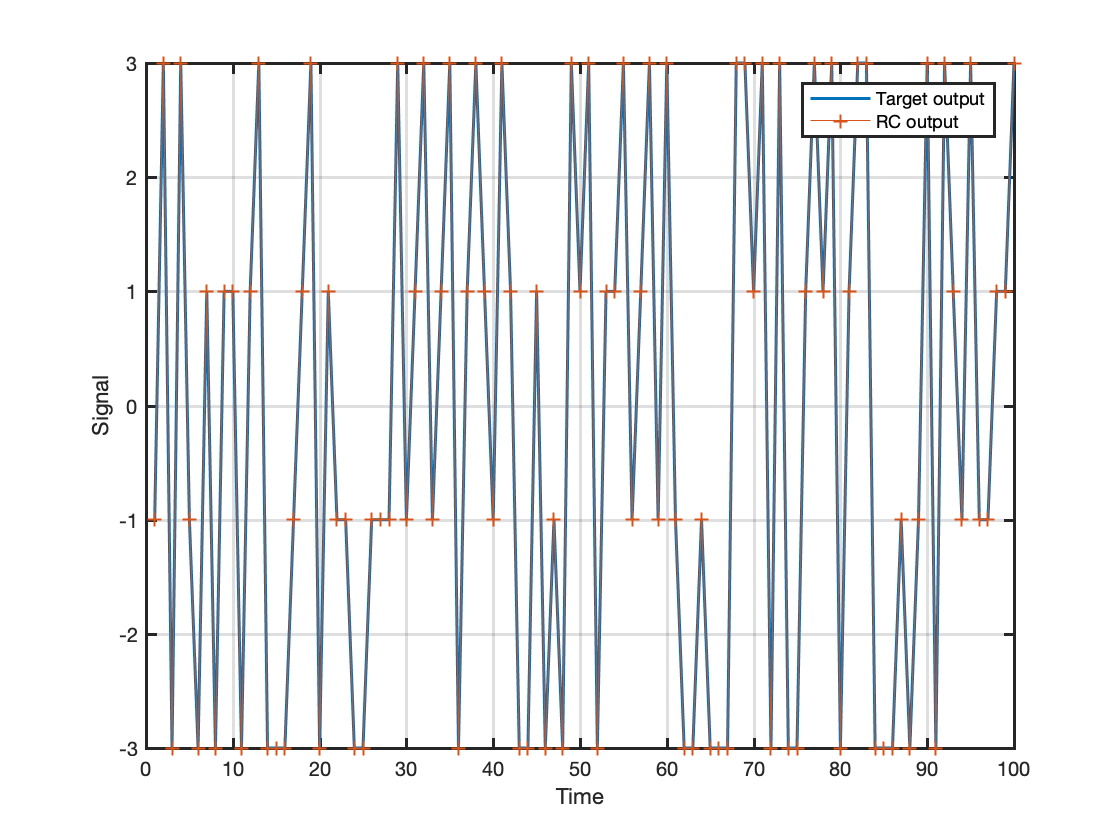
\includegraphics[width=\textwidth]{nonlinear_ch_eq}
	\caption{Nonlinear channel equalisation task with a signal error rate of $5~10^{-4}$, with signal to noise ratio equal to 32 dB. This reservoir is the same as the one in Figure \ref{narma10}, as well as the number of time steps for the washout, training and testing phases. The symbols predicted by the \rcer are found by changing the continuous valued output by the closest symbol.}
\end{figure}



